\chapter{Results} 
\label{chap:results}

% \begin{figure}[h]
%     \centering
%     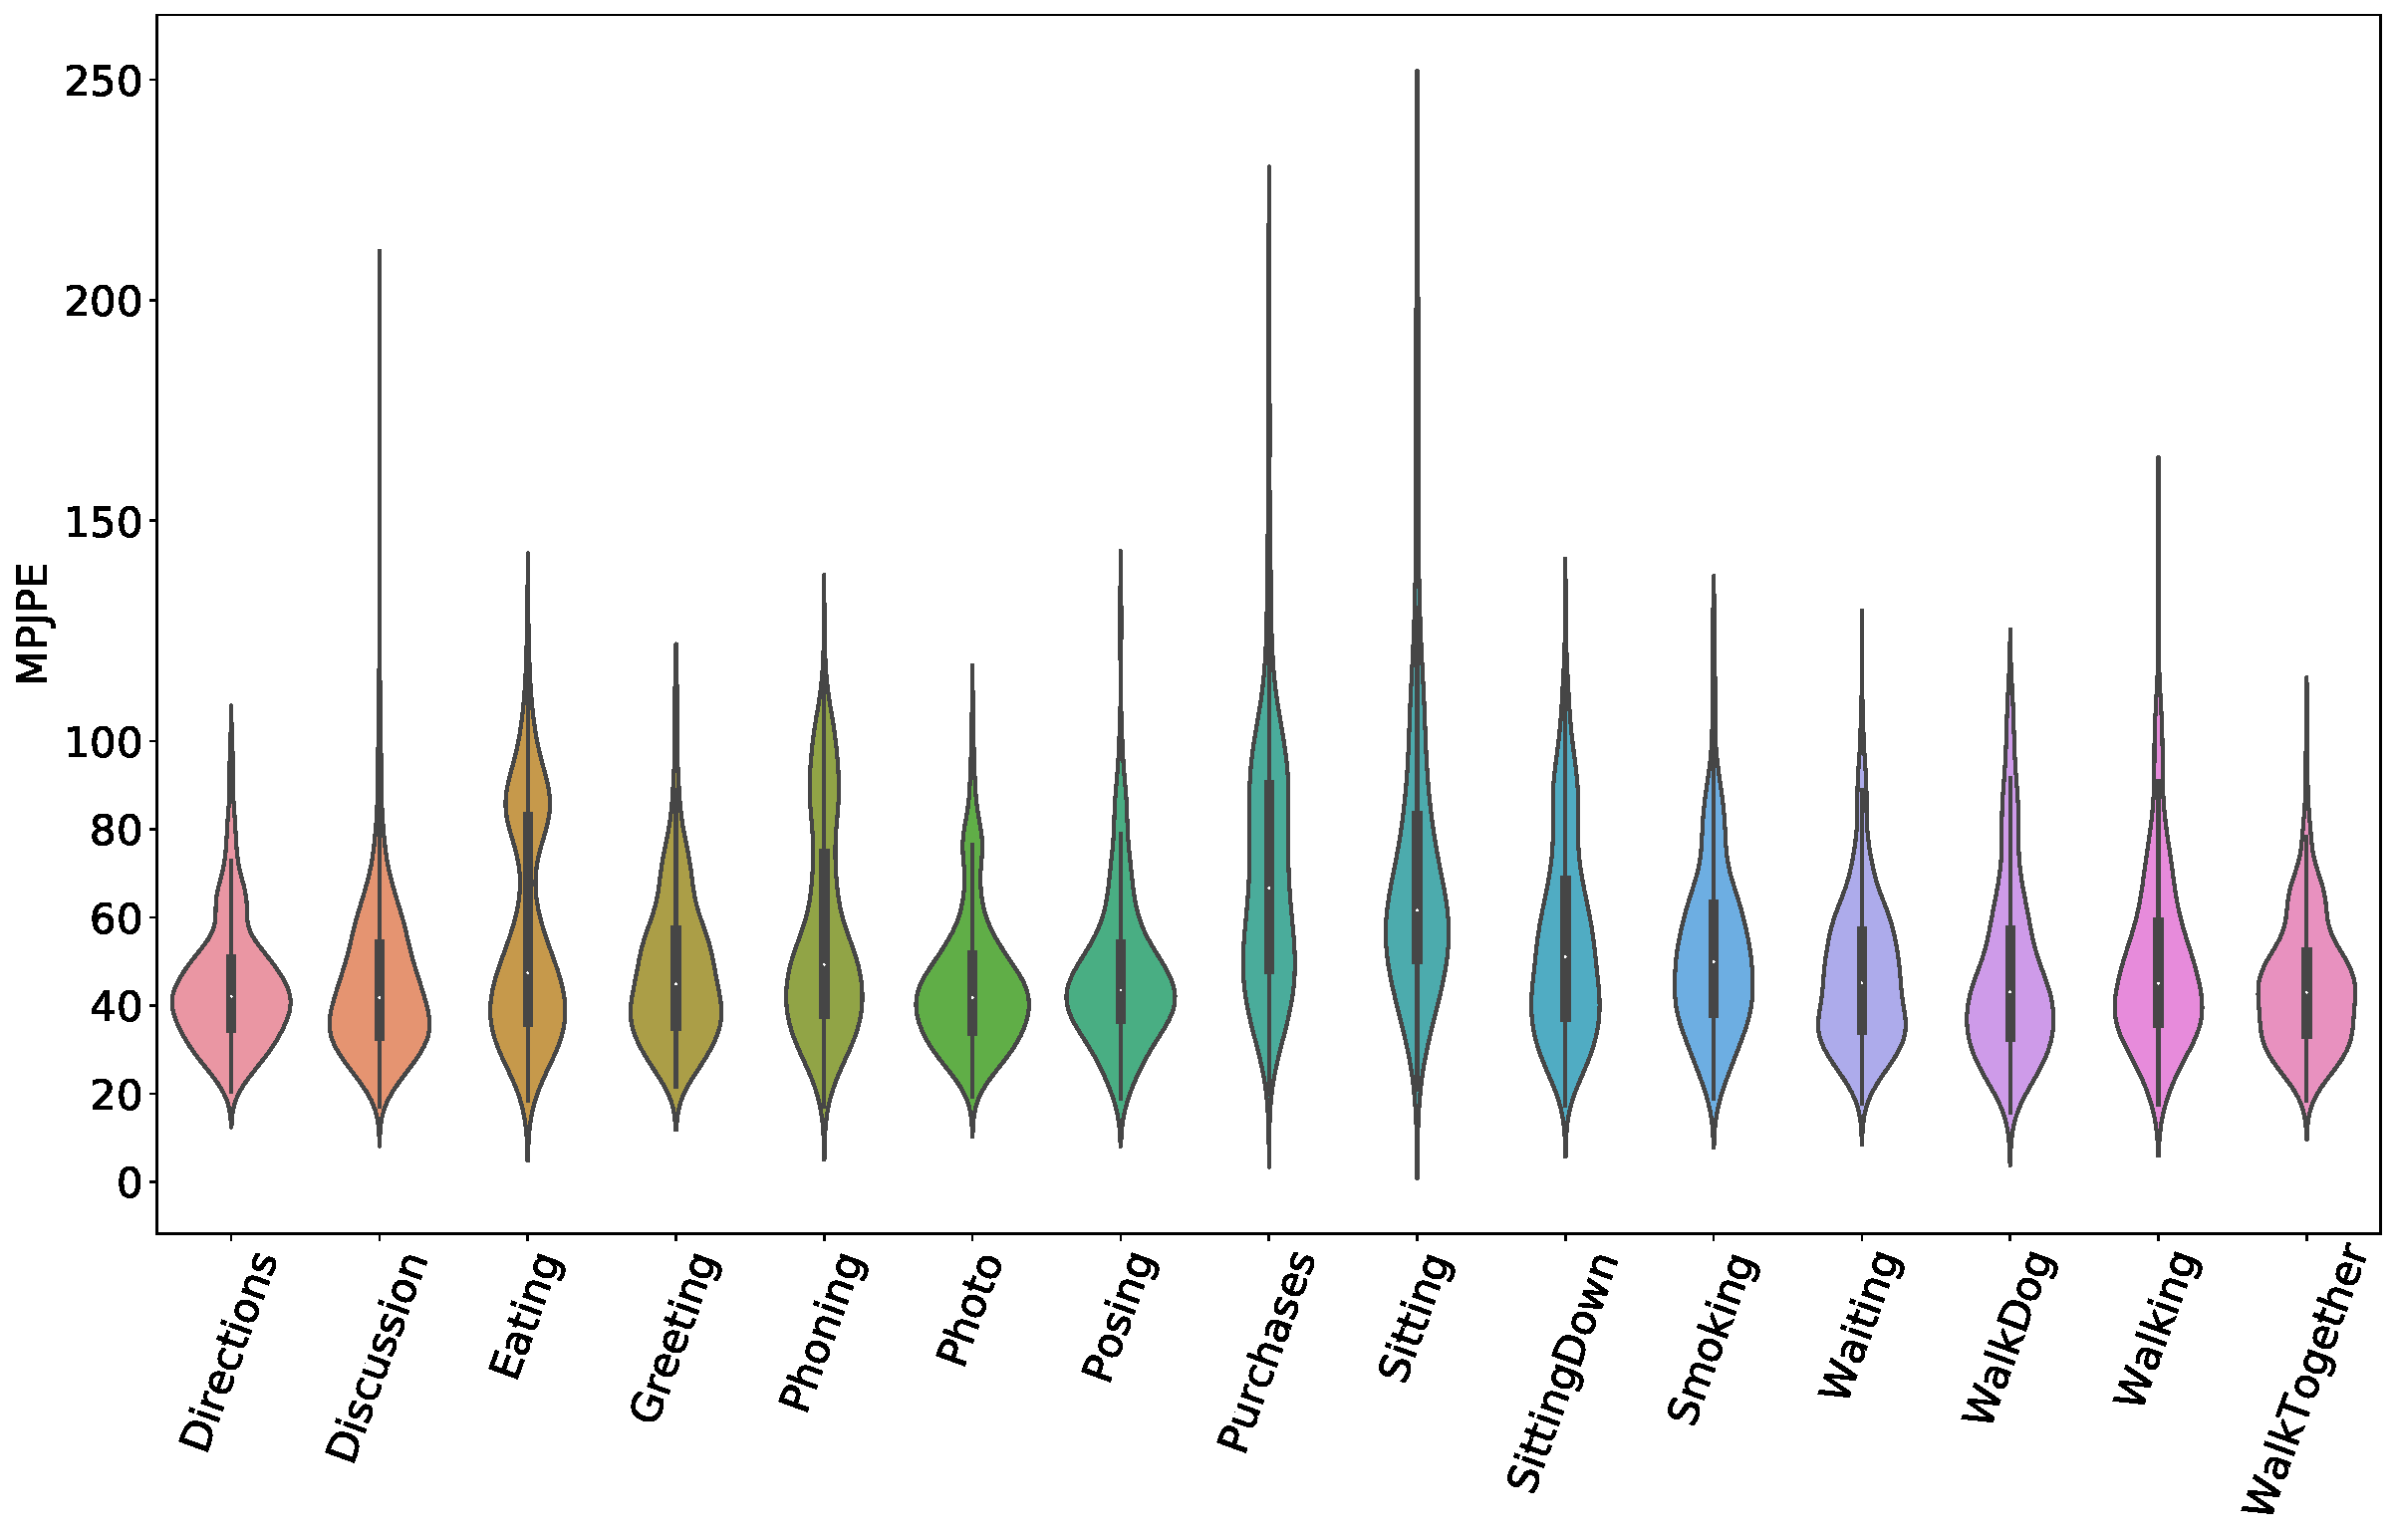
\includegraphics[width=\textwidth]{figures/results/violin_pjpe.pdf}
%     \caption{Visualization of the inputs and outputs of the model}
%     \label{fig:violin}
% \end{figure}

\section{missing joints}
\section{best hypothesis}

\section{Quantitative Results}

The results presented here are after training the networks for $\sim$400 epochs (~5.5 hours) on approximately 300,000 2D poses with a batch size of 2560 on an Nvidia Titan X. The input poses are flipped with a probability of 0.5. The model takes 16 joints as the output where the root is added at the origin for validation. The proposed architecture consists 1024 hidden units per linear layer and 51 latent dimensions. Both the \ac{vae} and the discriminator are trained using Adam optimizer with default hyperparameters and with a learning rate of 2e-4. The gradient norms of the discriminator is clipped to 1 when training the discriminator. While training the generator the gradient norms are clipped to 2 for all the models while the gradient values are clipped to 1000.

One of the challenging parts is finding the optimal weights for each of the terms in the triplet loss. The loss coefficients $\lambda_{recon}$, $\lambda_{\acs{kld}}$, $\lambda_{disc.}$ are set to 1, 0.001, 0.001 respectively. The higher weight is motivated by 2 reasons. $\lambda_{recon}$ refers to the constrained optimization and irrespective of how realistic it is, projection loss is desired to be consistently low to get better \ac{mpjpe}. That leads to the other reason that the quantitative results are given higher importance. 

The values of $\lambda{\acs{kld}}$ and $\lambda{disc.}$ can be tuned according to the task at hand based on how well the poses are to be clustered or how important it is to reject poses that are not realistic. The $\beta$ value for the \ac{vae} is cycled from 0 to $\lambda_{\acs{kld}}$ every 40 epochs. While keeping it constant at $\lambda_{\acs{kld}}$ for 10 epochs with a 10 epoch warmup at the beginning of the training. %TODO add loss standardization values to kld





The different poses during the training are presented in Fig. \ref{fig:sample_pred}. The poses in pink are the ground truth while the ones in blue are the predictions. The poses refer to ground truth 2D, reconstruction 2D, reconstruction novel view, reconstruction 3D, and combined reconstruction and ground truth 3D after alignment. The same order is followed for the other visualization. 

\begin{figure}[h]
    \centering
    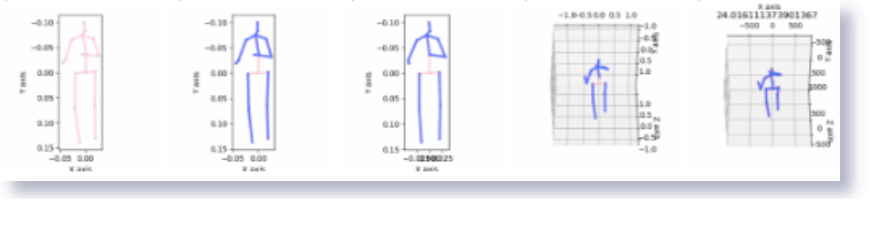
\includegraphics[scale=0.4]{figures/results/sample_pred.png}
    \caption{Visualization of the inputs and outputs of the model}
    \label{fig:sample_pred}
\end{figure}


The training is noise and the networks need to training for several hundreds of epochs before they tend to converge. The experiment which the results are from is trained over 1400 epochs but very slow improvements in the results are observed. At 1400 epochs the \ac{mpjpe} is $\sim$ 68 mm. This is far less than the current state of the art \cite{amazon1} with $\sim$ 40 mm. The results are believed to improve using \acp{wgan} as they offer better convergence. 

\begin{figure}[h]
    \centering
    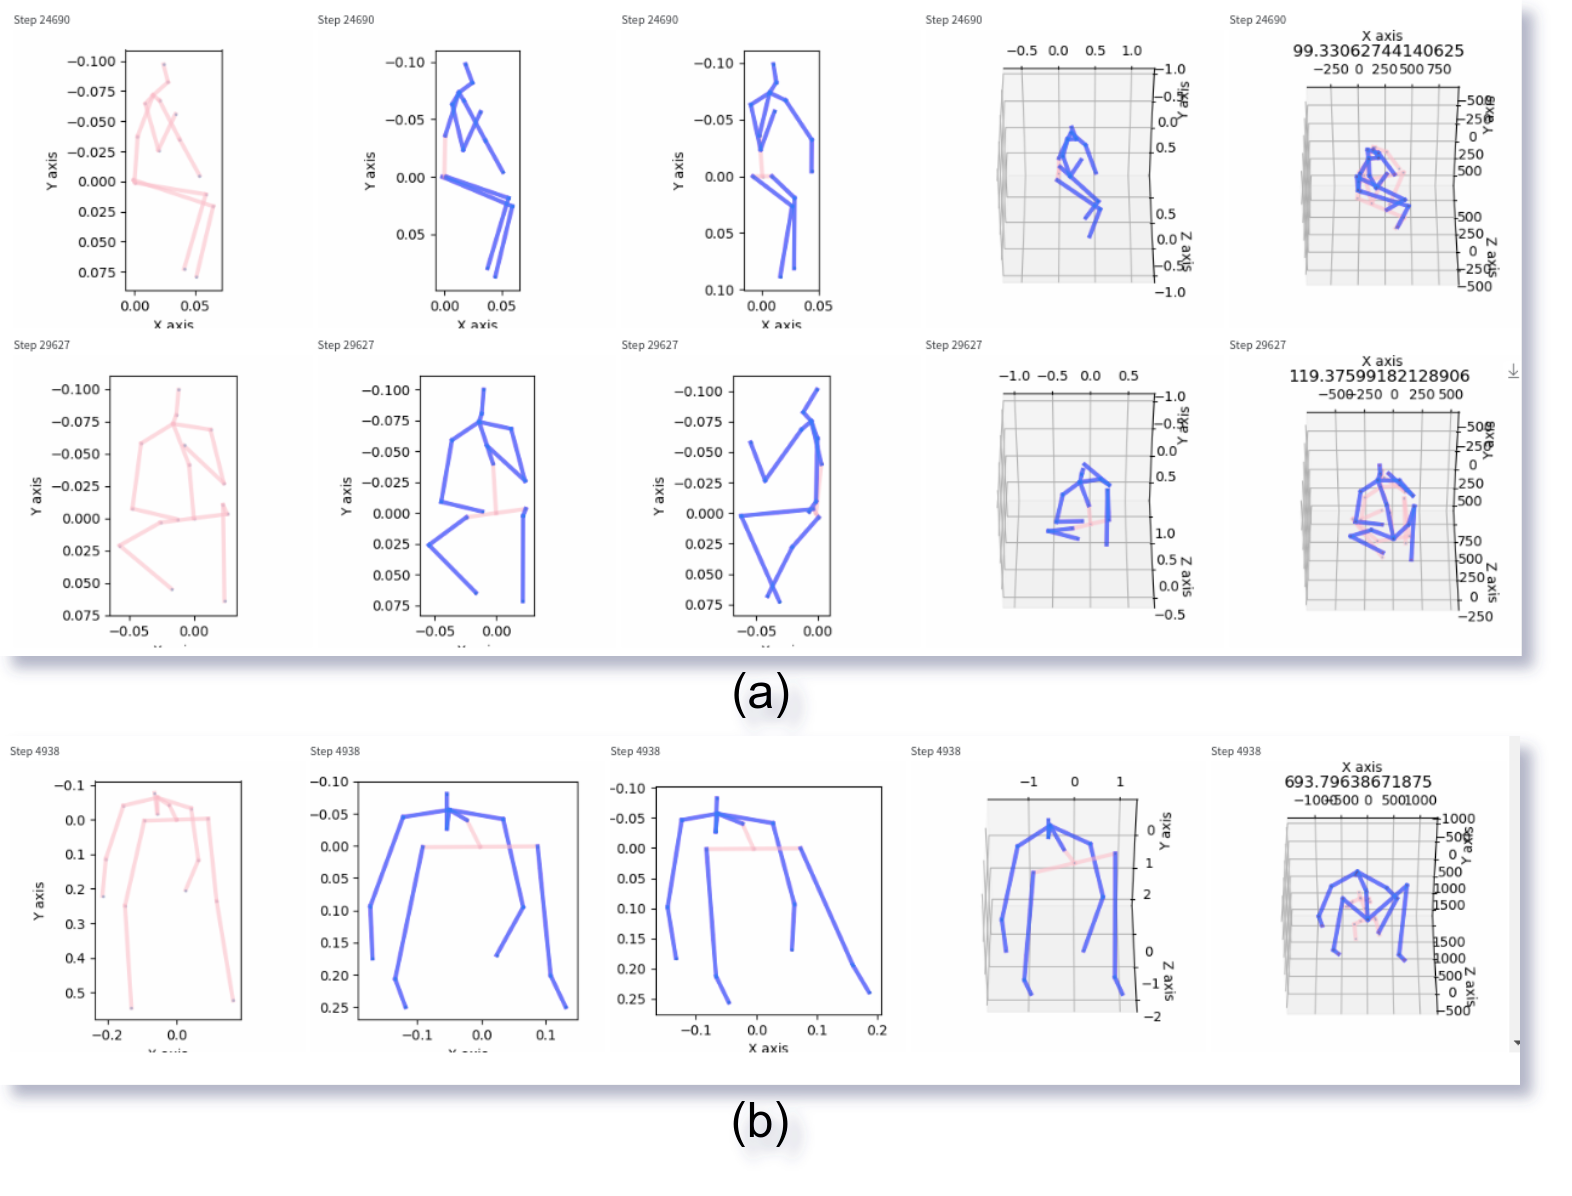
\includegraphics[scale=0.2]{figures/results/bad_samples.png}
    \caption{(a) Prediction on hard poses with hih ambiguity. (b) Poses that can be improved with changes to data processing.}
    \label{fig:bad_samples}
\end{figure}

Despite the \ac{mpjpe} being $\sim$ 68, the decoder generates many accurate 3D poses that are almost indistinguishable for the human eye. The high number of outliers and lower performance on hard poses worsens the overall performance of the model. The graph on the left depicted in fig \ref{fig:mpjpe_trends} shows the slow and gradual decrease in \ac{mpjpe}. And the graph on the right shows the histogram of the \ac{pjpe} of each sample over time. This shows the model is unable to certain poses while it improves gradually on the rest. 

\begin{figure}[h]
    \centering
    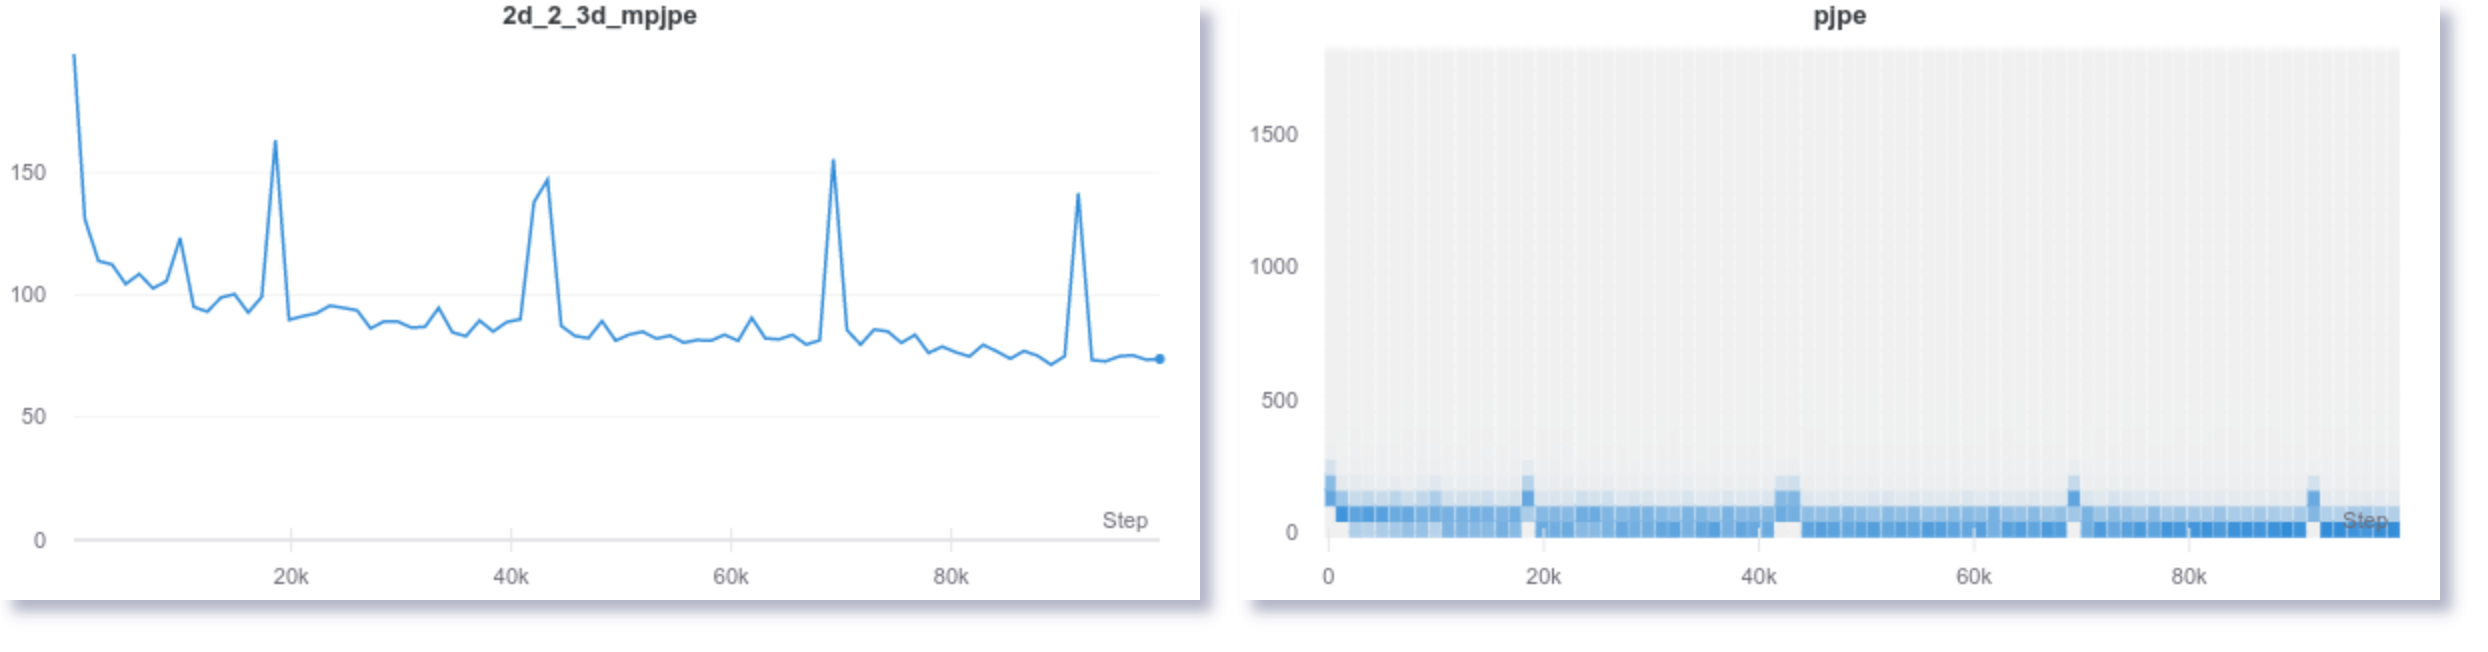
\includegraphics[scale=0.2]{figures/results/mpjpe_trend.png}
    \caption{MPJPE and PJPE trends during the training respectively}
    \label{fig:mpjpe_trends}
\end{figure}

Some of such outliers are presented in fig \ref{fig:bad_samples}, the predictions in (a) are the ones the model is unable to learn. While (b) is the evidence of the shortcoming of the current processing technique. Rectifying that would improve the evaluation metric of the model quite significantly.



The visualization of 2D pose embedding in latent space after dimensionality reduction using \ac{umap} is shown in fig. \ref{fig:latentspace}. Each action is given a unique color. Though we small clusters of blues, browns, pinks the overall space looks very mixed up. This is expected as many of the instances in different actions overlap. For example, the action standing up and sitting down have instances while both or standing or sitting, etc.  

\begin{figure}[h]
    \centering
    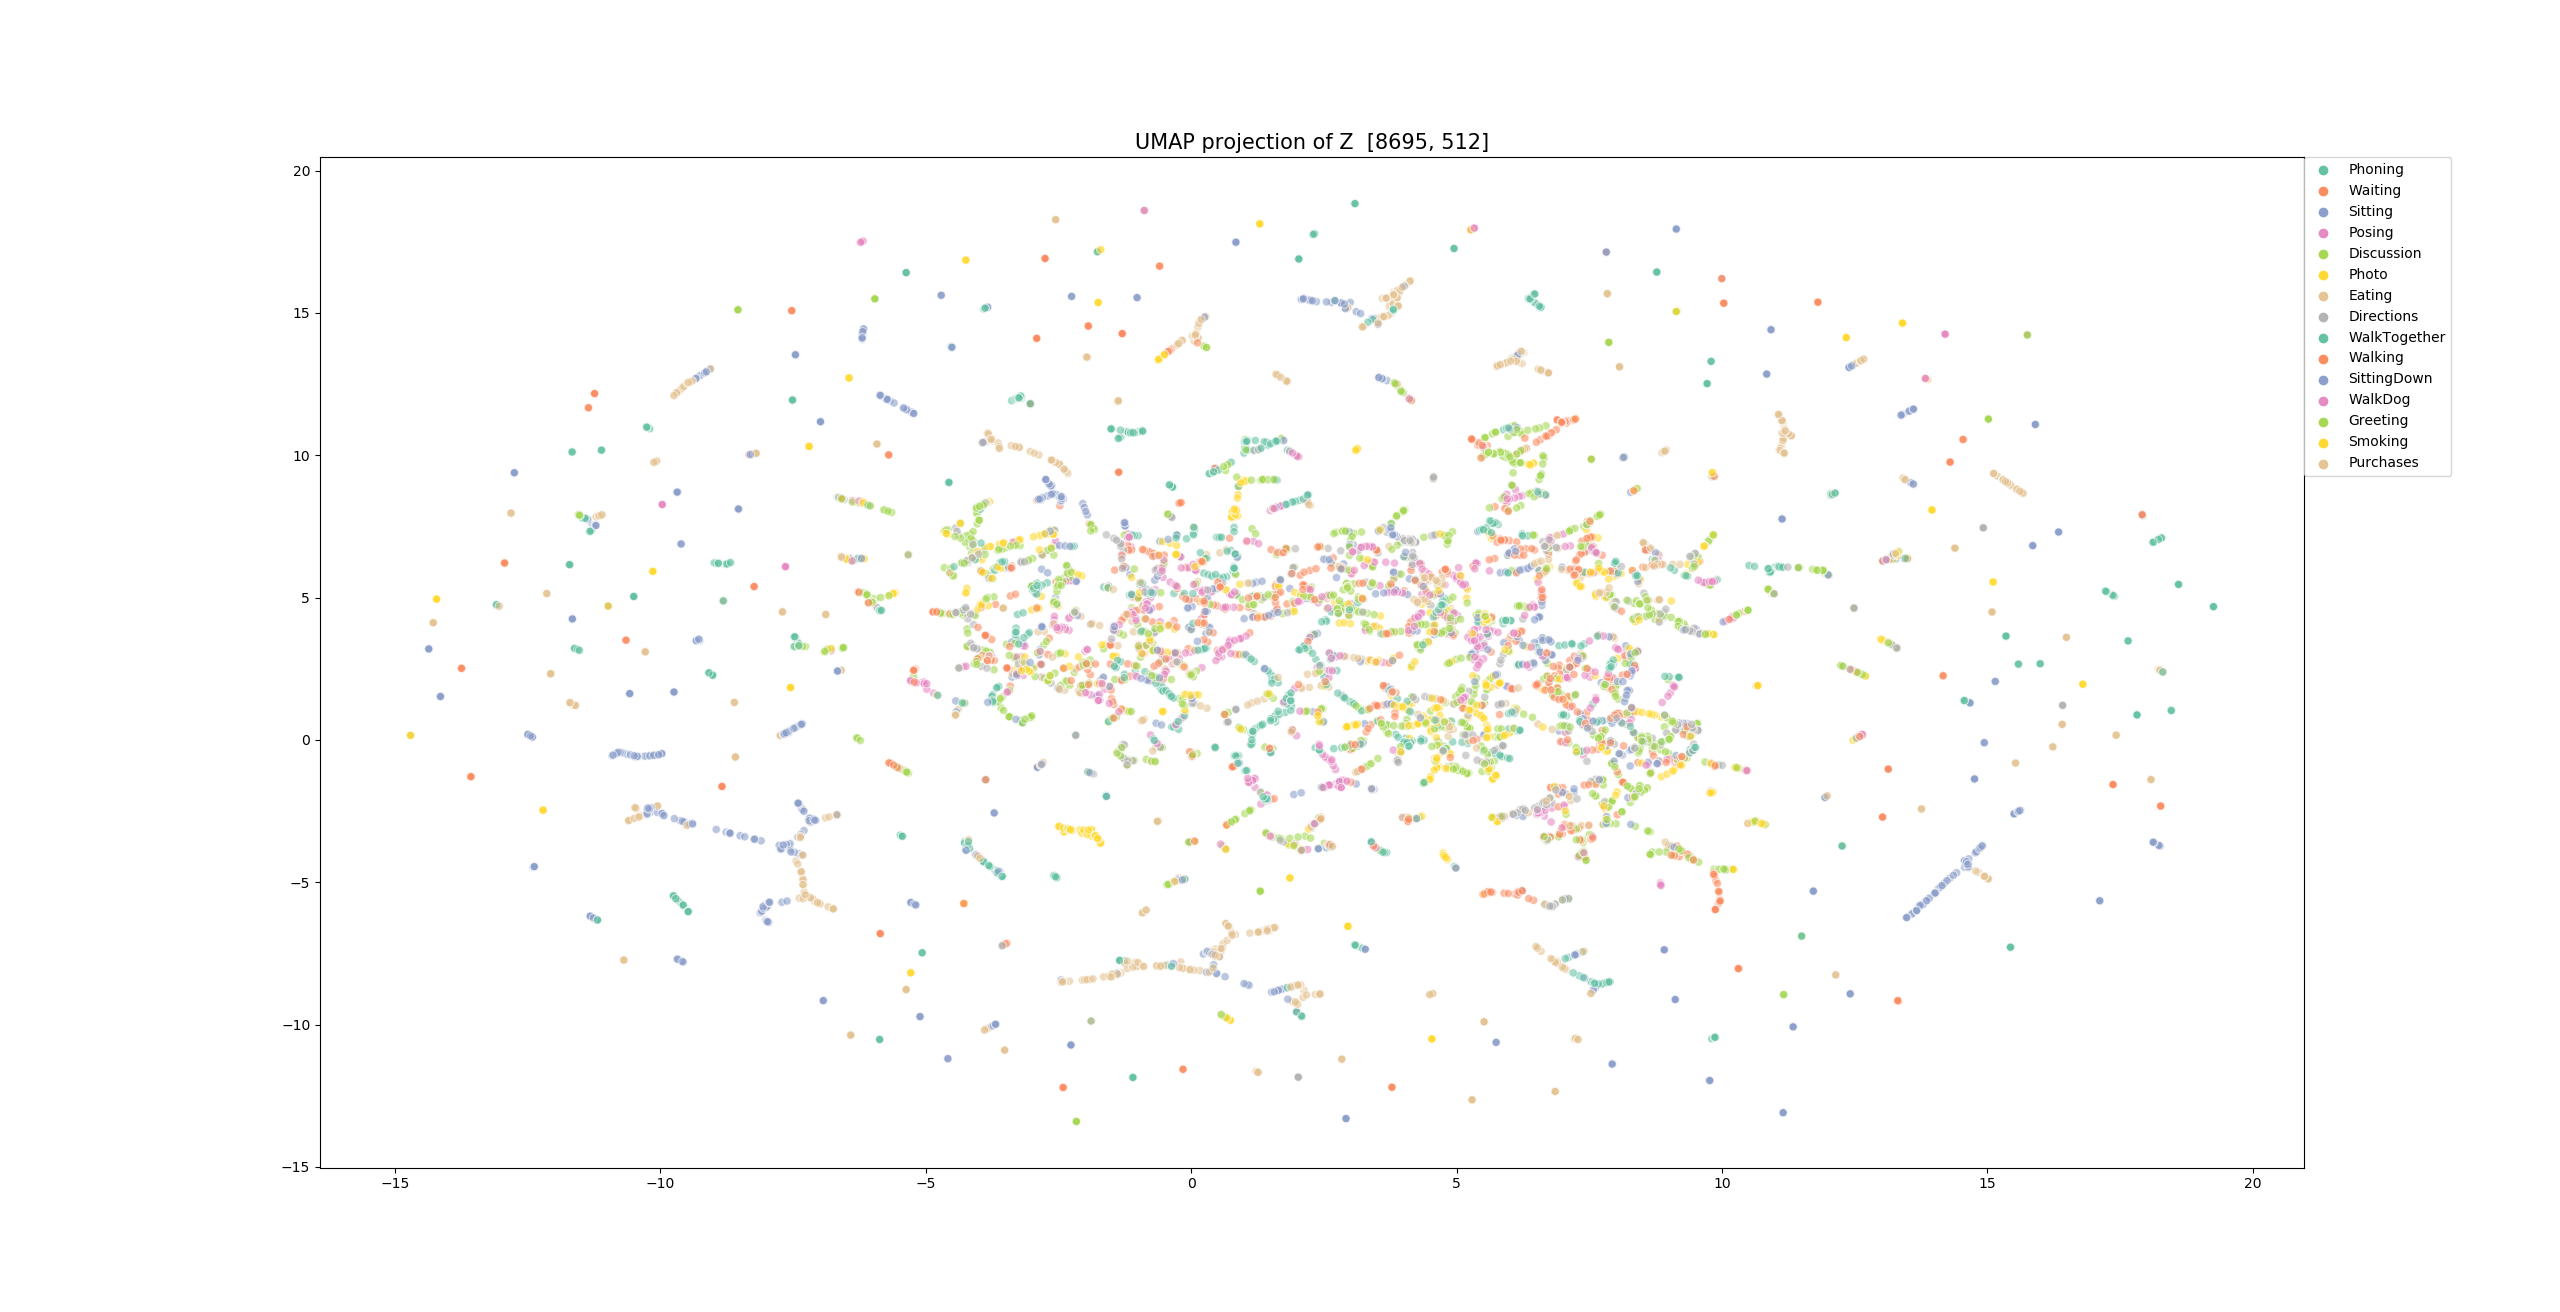
\includegraphics[width=\textwidth]{figures/results/umap.png}
    \caption{UMAP Visualization of samples in latent space. The actions do not always directly related to the pose due to overlaps from one action to another. Better viewed in color and 200\% zoom}
    \label{fig:latentspace}
\end{figure}